\documentclass[11pt,a4paper]{article}

\usepackage[T1]{fontenc}
\usepackage{lmodern}
\usepackage[margin=2.4cm]{geometry}
\usepackage{microtype}
\usepackage{amsmath,amssymb}
\usepackage{graphicx}
\usepackage{booktabs}
\usepackage{tabularx}
\usepackage{float}
\usepackage{xcolor}
\usepackage{tikz}
\usetikzlibrary{arrows.meta,positioning,fit,backgrounds}
\usepackage[numbers,sort&compress]{natbib}
\usepackage[colorlinks=true,linkcolor=blue!50!black,citecolor=blue!50!black,urlcolor=blue!50!black]{hyperref}

\graphicspath{{../figures/}}
\newcommand{\doop}{\operatorname{do}}
\newcolumntype{Y}{>{\raggedright\arraybackslash}X}
\setlength{\parskip}{0.35em}

\title{\textbf{Neuro-Symbolic Causal Inference via Language Model\\Knowledge Extraction and Bayesian Networks}}
\author{\textbf{Team T013}\\[0.6em]
\small
\begin{tabular}{@{}ll@{}}
Divyansh Rathore & 2401020021 \\
Arya & 2401020012 \\
Krishna Dave & 2401010238 \\
Rishita Boisnobi & 2401010382 \\
Vriha Dholiya & 2401010508 \\
\end{tabular}}
\date{October 2026}

\begin{document}
\maketitle

\begin{abstract}
\noindent
We build a system that extracts candidate cause--effect relations from text, assembles them into a directed acyclic graph (DAG), and
uses a Bayesian network fitted to real survey data to answer interventional queries. Two extractors are compared on the same task: a
rule-based baseline over spaCy dependency parses, and a fine-tuned DistilBERT relation classifier. On the held-out SemEval-2010 Task 8
test set, DistilBERT clearly outperforms the rules (F1 0.91 vs.\ 0.74, non-overlapping bootstrap intervals). Applied to 500 PubMed
abstracts on smoking and lung disease, the picture changes. DistilBERT's precision falls to 0.45 against silver labels, its graph needs
59 edges removed to become acyclic, and it proposes arrows that reverse established facts, while the rules remain precise (0.79) but
recall only 0.15. Retraining DistilBERT with 780 labelled PubMed pairs, taking every pair of each sentence and splitting by abstract,
raises its PubMed F1 from 0.43 to 0.54 and halves its false alarms, while its SemEval test F1 stays at 0.92. Against 14 conclusions of the US Surgeon General, the rule graph has an edge precision of 0.58 with no contradictions,
and the DistilBERT graph 0.22 with two. A Bayesian network over the extracted structure, fitted to 16{,}904 NHANES adults with age as a
confounder, answers six documented $\doop$-queries (e.g.\ a 9.3$\times$ causal risk ratio of smoking on COPD) in agreement with the
published evidence. A single reversed arrow, \textit{COPD $\rightarrow$ smoking}, which DistilBERT supported in 33 abstracts, would change
that answer to 1.0 (no effect), even though both graphs fit the data equally well. Fluent text extraction is therefore not sufficient for
causal reasoning; the symbolic stage is what makes the answers consistent.
\end{abstract}

\section{Introduction}

Scientific and news text is full of causal claims (``smoking is the leading cause of COPD''). Language models are good at
recognising such statements, but a collection of extracted sentences is not a causal model. Text extraction alone cannot
(i)~guarantee that the extracted relations form an acyclic structure, (ii)~quantify uncertainty in a calibrated way, or
(iii)~answer intervention queries such as ``how would COPD prevalence change if nobody smoked?'' consistently. Answering such
queries requires a causal graph and the machinery of Bayesian networks and the $\doop$-operator~\citep{pearl1988,pearl2009}.

This project separates the two jobs in a \emph{neuro-symbolic} pipeline (Figure~\ref{fig:pipeline}). A \textbf{neural} stage reads text
and proposes candidate (cause, effect) triples. A \textbf{symbolic} stage merges them into a DAG with evidence on every edge, removes
self-loops and cycles, tests the graph against data, fits a Bayesian network, and answers interventional queries.

\textbf{Contributions.}
\begin{itemize}
  \item A reproducible pipeline from text to interventional answers, combining SemEval-2010 Task 8 for training and scoring the
        extractors, PubMed abstracts for building the graph, and NHANES survey data for the probabilities.
  \item A fair comparison of a rule-based (AML) extractor and a fine-tuned DistilBERT model on identical inputs, scored both on a
        labelled in-domain test set and on scientific text.
  \item A separate evaluation of the resulting graphs, by edge precision against cited Surgeon General conclusions and by the effect of the
        graph structure on causal answers.
  \item A targeted fix for the DL model's domain shift: retraining with labelled PubMed pairs, several per sentence and split by
        abstract, evaluated on the same held-out pairs as before.
\end{itemize}

\begin{figure}[t]
\centering
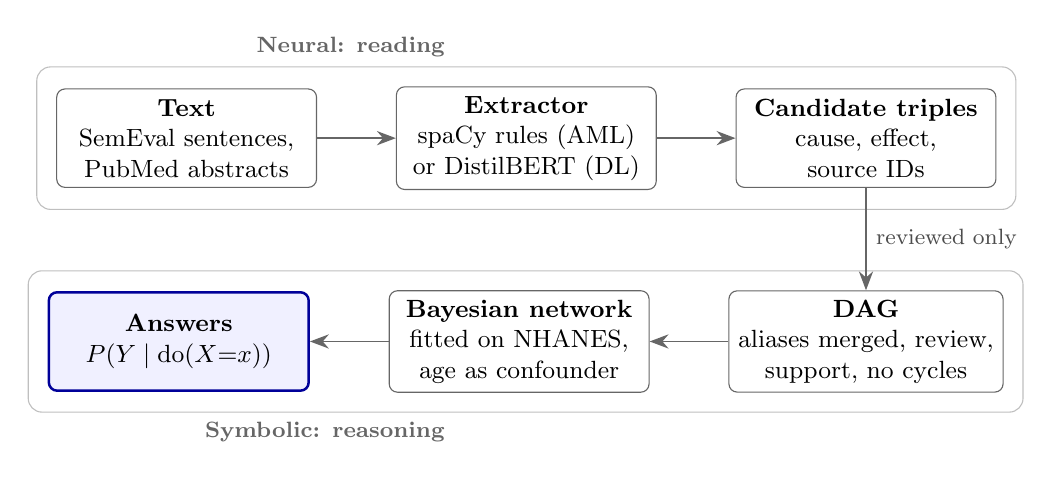
\begin{tikzpicture}[
  box/.style={draw=black!60, rounded corners=3pt, minimum width=3.3cm, minimum height=1.25cm, align=center, font=\small},
  key/.style={box, draw=blue!60!black, fill=blue!6, line width=0.9pt},
  arr/.style={-{Stealth[length=2.4mm]}, black!60, line width=0.7pt},
  grp/.style={draw=black!25, rounded corners=5pt, inner sep=7pt}]
  \node[box] (text) {\textbf{Text}\\SemEval sentences,\\PubMed abstracts};
  \node[box, right=1.0cm of text] (ext) {\textbf{Extractor}\\spaCy rules (AML)\\or DistilBERT (DL)};
  \node[box, right=1.0cm of ext] (trip) {\textbf{Candidate triples}\\cause, effect,\\source IDs};
  \node[box, below=1.3cm of trip] (dag) {\textbf{DAG}\\aliases merged, review,\\support, no cycles};
  \node[box, left=1.0cm of dag] (bn) {\textbf{Bayesian network}\\fitted on NHANES,\\age as confounder};
  \node[key, left=1.0cm of bn] (ans) {\textbf{Answers}\\$P(Y \mid \doop(X{=}x))$};
  \draw[arr] (text) -- (ext);
  \draw[arr] (ext) -- (trip);
  \draw[arr] (trip) -- node[right, font=\footnotesize, black!70] {reviewed only} (dag);
  \draw[arr] (dag) -- (bn);
  \draw[arr] (bn) -- (ans);
  \begin{scope}[on background layer]
    \node[grp, fit=(text)(ext)(trip), label={[font=\footnotesize\bfseries, black!60]above left:Neural: reading}] {};
    \node[grp, fit=(ans)(bn)(dag), label={[font=\footnotesize\bfseries, black!60]below left:Symbolic: reasoning}] {};
  \end{scope}
\end{tikzpicture}
\caption{The neuro-symbolic pipeline. The language side proposes relations; the symbolic side enforces structure and answers
interventional queries.}
\label{fig:pipeline}
\end{figure}

\section{Background}

\textbf{Bayesian networks and interventions.} A Bayesian network is a DAG $G$ over variables $V$ together with conditional
probability tables, factorising $P(V)=\prod_{v} P(v \mid \mathrm{pa}(v))$~\citep{pearl1988}. Under a causal reading of $G$, the
intervention $\doop(X{=}x)$ removes all arrows into $X$ and fixes its value (\emph{graph surgery}). When a set $Z$ blocks every
back-door path from $X$ to $Y$, the interventional distribution is identified by the adjustment formula~\citep{pearl2009}
\begin{equation}
  P\big(Y \mid \doop(X{=}x)\big) = \sum_{z} P(Y \mid X{=}x, Z{=}z)\, P(Z{=}z),
  \label{eq:backdoor}
\end{equation}
which in general differs from the observational $P(Y \mid X{=}x)$. The direction of every arrow matters: it decides which
variables are adjusted for, and whether $Y$ is affected by $X$ at all.

\textbf{Transformers for relation extraction.} BERT~\citep{devlin2019} learns contextual representations by pre-training on large
corpora; DistilBERT~\citep{sanh2019} is a distilled version with 40\% fewer parameters that keeps most of BERT's accuracy. For
relation classification, the two arguments are commonly marked with special tokens in the input~\citep{baldinisoares2019}.

\textbf{Datasets considered.} Corr2Cause~\citep{jin2024corr2cause}, the suggested starter dataset, tests whether causal claims follow
from correlation statements over abstract variables (``A correlates with B''). It contains no natural-language entities to extract, so
we used SemEval-2010 Task 8~\citep{hendrickx2010} for extraction, which annotates the relation between two marked nominals in natural
sentences.

\section{Data}

\begin{table}[H]
\centering\small
\begin{tabularx}{\linewidth}{@{}lYl@{}}
\toprule
Source & Role in the pipeline & Size used \\
\midrule
SemEval-2010 Task 8~\citep{hendrickx2010} & Train, tune and test both extractors & 10{,}698 sentences (12.5\% causal) \\
PubMed (E-utilities API) & Text the causal graph is built from & 500 abstracts, 5{,}185 sentences \\
NHANES 2013--2018 + linked mortality~\citep{nhanes,nchsmort} & Probabilities for the Bayesian network & 16{,}904 adults \\
US Surgeon General reports~\citep{sgr2014,sgr2010} & Reference facts for graph evaluation & 14 causal conclusions \\
\bottomrule
\end{tabularx}
\caption{Data sources.}
\label{tab:data}
\end{table}

\textbf{SemEval.} Each sentence marks two entities and carries one of 19 labels (nine relation types in both directions, plus
\textit{Other}). The two \textit{Cause-Effect} labels are positives; for \textit{Cause-Effect(e2,e1)} the arrow is flipped so that
(cause, effect) is always explicit. All other labels are negatives, which provides hard ``related but not causal'' examples. The
official test set (2{,}717 sentences, 328 causal) is kept untouched until the final comparison; 15\% of the official training set,
stratified by label, forms the validation set (1{,}195 sentences). A leakage check found 19 sentences duplicated across splits, and
they were removed from train/validation, leaving 6{,}786 training sentences (852 causal).

\textbf{PubMed.} We retrieved the 500 most relevant abstracts (published 2010--2024) for a query combining smoking with lung disease
(COPD, emphysema, lung cancer) and cached them, so the corpus is fixed.

\textbf{NHANES.} Three survey cycles (2013--2018) were pooled and linked to the NCHS public-use mortality files (deaths up to 31 Dec
2019). Variables: age group (20--44 / 45--64 / 65+), smoking (never / former / current, from SMQ020 and SMQ040), self-reported
doctor-diagnosed COPD (664 cases), emphysema (324), chronic bronchitis (1{,}003), lung cancer (54), and all-cause death during follow-up (872).

\section{Methods}

\subsection{Task, entity schema and triples}

Both extractors solve the same task: given a sentence and two marked entities, predict \texttt{e1$\rightarrow$e2},
\texttt{e2$\rightarrow$e1} or \texttt{none}. Every positive prediction becomes a \texttt{CausalTriple}(cause, effect, document ID,
sentence ID, source, confidence). The record normalises names (lower-case, leading determiners removed) and rejects self-loops at
construction time.

For PubMed we defined a small \textbf{entity schema} of 20 concepts in three groups: exposures (smoking, secondhand smoke,
e-cigarettes, smoking cessation, air pollution), mechanisms (inflammation, oxidative stress, apoptosis, senescence, infection), and
diseases/outcomes (COPD, emphysema, chronic bronchitis, asthma, pulmonary fibrosis, lung cancer, airflow obstruction, lung-function
decline, exacerbations, mortality). Each concept lists its aliases (\textit{smokers}, \textit{cigarette smoke}, \textit{CS exposure}
$\rightarrow$ \texttt{smoking}). These are matched case-insensitively, with the longest match winning. An ignore list removes false friends:
``cell \emph{death}'' is not mortality. Bare ``fibrosis'' was excluded after inspection, because it often meant airway fibrosis. Every pair of
different concepts within one sentence is a candidate (6{,}051 pairs in 2{,}085 sentences) and is stored with entity markers, so both
extractors label exactly the same pairs.

\subsection{AML baseline: dependency rules}

Rules walk the dependency path between the two entity heads (via their lowest common ancestor) and fire on a causal trigger with a
grammatical pattern that also fixes the direction. There are eight patterns: active verb (\textit{X causes Y}), relative clause
(\textit{X that leads to Y}), passive (\textit{Y was caused by X}), participle (\textit{Y caused by X}), ``from''-verbs
(\textit{Y stems from X}), cause nouns (\textit{X is a cause of Y}), result nouns (\textit{Y is the result of X}) and a bare
\textit{from}. We started from 24 trigger verbs and 12 trigger nouns chosen by intuition. A trigger was then kept only if its precision
on the \emph{training} split was at least 0.5. This removed, for example, \textit{make} (7\%), \textit{produce} (25\%) and
\textit{from} (43\%), which mostly signal Product-Producer and Entity-Origin relations, and kept nine triggers (\textit{arise, cause,
contribute, generate, lead, reason, result, stem, trigger}).

\subsection{DL model: fine-tuned DistilBERT}\label{sec:dl}

We fine-tuned \texttt{distilbert-base-uncased}~\citep{sanh2019,wolf2020} as a three-way sequence classifier over the marked sentence,
adding \texttt{<e1>}, \texttt{</e1>}, \texttt{<e2>}, \texttt{</e2>} as special tokens~\citep{baldinisoares2019}. Training used
AdamW~\citep{loshchilov2019} (learning rate $5\times10^{-5}$, weight decay 0.01, batch size 32, linear decay after 10\% warm-up,
gradient clipping at 1.0) for four epochs. The epoch with the best validation F1 was kept. Training took about 20 minutes on an Apple M3 GPU.
The softmax probability of the predicted class is stored as the triple's confidence.

\subsection{From triples to a DAG}

Triples from one extractor are merged into a weighted directed graph. The same fact stated twice in one sentence counts once, and
every edge records its supporting abstracts and sentences. Support is counted in \emph{abstracts}, so that one paper repeating a claim
does not outweigh independent papers. Following the brief, only reviewed predictions should reach the graph: every edge is exported
with an example sentence to a review file, and edges a reviewer marks \textit{no} are removed. Edges supported by fewer than two
abstracts are then dropped. Finally, while a cycle remains, its weakest edge (fewest abstracts, then fewest sentences, then a fixed
order) is removed and logged.

\subsection{Bayesian network}

The network uses every text-DAG edge whose endpoints are both measured in NHANES (11 edges; 8 edges touching unmeasured mechanisms
are left out), plus \emph{age $\rightarrow$ every node}. Age is not in the entity schema, so no extracted edge mentions it, but it is a known
confounder of smoking history and disease. It was added from domain knowledge and documented as such. Before fitting, the structure
is tested in two ways: BIC scores~\citep{schwarz1978} of alternative graphs, and chi-square tests of the conditional independences the
graph implies. Conditional probability tables are estimated with a BDeu prior (equivalent sample size 10)~\citep{heckerman1995}, because
some parent configurations are rare. Observational queries use variable elimination; interventional queries use pgmpy's causal
inference engine~\citep{ankan2015}, which applies the back-door adjustment~\eqref{eq:backdoor} (here $Z=\{\text{age}\}$).

\subsection{Evaluation protocol}

Extraction and the graph are evaluated separately, as the brief requires.

\textbf{Extraction metrics.} Precision, recall and F1 on the causal class; a prediction counts as correct only if it is causal
\emph{and} has the correct direction. 95\% intervals for F1 come from 1{,}000 bootstrap resamples~\citep{efron1979}.

\textbf{PubMed silver labels.} PubMed has no gold labels, so an instruction model (Claude) labelled a sample. This is permitted by the
brief (``a carefully evaluated instruction model''). A written guideline was fixed first: a pair is causal only if the sentence
\emph{claims} that one concept causes, leads to, contributes to or raises the risk of the other, and mere association is not causal. Labelling
was blind to both extractors' predictions. To evaluate the labeller, it first labelled 150 SemEval test sentences (75 causal, 75 not)
without seeing their human labels. The PubMed sample is stratified by the extractors' agreement (both causal / rules only / DistilBERT
only / neither; 60, 20, 110 and 110 pairs). Each labelled pair carries weight $w_s = N_s / n_s$, the stratum size divided by the number
sampled, so that weighted counts estimate performance over all 6{,}051 pairs:
\begin{equation}
  \widehat{P} = \frac{\sum_i w_i\,[\hat y_i = y_i \neq \text{none}]}{\sum_i w_i\,[\hat y_i \neq \text{none}]},\qquad
  \widehat{R} = \frac{\sum_i w_i\,[\hat y_i = y_i \neq \text{none}]}{\sum_i w_i\,[y_i \neq \text{none}]}.
\end{equation}
Bootstrap resampling is done within strata.

\textbf{Graph metrics.} Each edge is judged by fixed rules against 14 causal conclusions drawn from the US Surgeon General's
reports~\citep{sgr2014,sgr2010}. An edge is \emph{established} if it matches a conclusion (e.g.\ smoking $\rightarrow$ COPD: ``the evidence
is sufficient to infer that smoking is the dominant cause of COPD''). It \emph{contradicts} if it reverses an established edge, makes
mortality a cause, or makes anything cause an exposure. Otherwise it is \emph{unverified}. Edge precision is the share of established edges.

\section{Results}

\subsection{Extraction on SemEval}

\begin{table}[H]
\centering\small
\begin{tabular}{@{}lccccc@{}}
\toprule
 & \multicolumn{3}{c}{Validation} & \multicolumn{2}{c}{Test (held out)} \\
\cmidrule(lr){2-4}\cmidrule(l){5-6}
Extractor & P & R & F1 & P / R & F1 [95\% CI] \\
\midrule
Rules, all triggers & 0.56 & 0.63 & 0.59 & -- & -- \\
Rules, pruned triggers & \textbf{0.94} & 0.49 & 0.65 & \textbf{0.94} / 0.61 & 0.74 [0.69, 0.78] \\
DistilBERT & 0.88 & \textbf{0.89} & \textbf{0.88} & 0.90 / \textbf{0.91} & \textbf{0.91} [0.88, 0.93] \\
\bottomrule
\end{tabular}
\caption{Directional extraction scores on SemEval. Pruning the trigger list on the training split raised the rules' validation
precision from 0.56 to 0.94.}
\label{tab:semeval}
\end{table}

DistilBERT's validation F1 rose from 0.83 (epoch~1) to 0.88 (epoch~3) and stayed level in epoch~4, while the training loss kept
falling (0.32 $\rightarrow$ 0.015), the usual onset of overfitting. On validation, DistilBERT recovered 59 causal sentences the rules
missed and missed none that the rules found. Neither model predicted a wrong direction on a causal validation sentence. The rules'
misses involve phrasing outside the trigger list (\textit{turning into}), pruned ambiguous cues (\textit{headaches from mold}) and
implied causation. On the test set, the bootstrap intervals do not overlap (Table~\ref{tab:semeval}).

\subsection{Labeller check and extraction on PubMed}

Against SemEval's human labels, the labeller agreed on 96.0\% of 150 sentences (Cohen's $\kappa = 0.93$~\citep{cohen1960}), with precision
1.00 and recall 0.92. All six disagreements were borderline SemEval conventions labelled \textit{none} (e.g.\ ``radiation \emph{from}
the microwaves''). Of the 300 PubMed pairs, 129 were labelled causal.

\begin{table}[H]
\centering\small
\begin{tabular}{@{}lccccrrrr@{}}
\toprule
 & \multicolumn{4}{c}{Scores} & \multicolumn{4}{c}{Estimated pairs (of 6{,}051)} \\
\cmidrule(lr){2-5}\cmidrule(l){6-9}
 & P & R & F1 & F1 95\% CI & correct & wrong dir. & false alarm & missed \\
\midrule
Rules & \textbf{0.79} & 0.15 & 0.25 & [0.20, 0.32] & 223 & 13 & \textbf{47} & 1{,}275 \\
DistilBERT & 0.45 & \textbf{0.42} & \textbf{0.43} & [0.36, 0.52] & \textbf{628} & 23 & 744 & \textbf{860} \\
\bottomrule
\end{tabular}
\caption{PubMed extraction against silver labels, weighted to all 6{,}051 candidate pairs. The right block estimates how many of all candidate pairs fall into each outcome.}
\label{tab:pubmed}
\end{table}

\textbf{Domain shift.} DistilBERT's precision falls from 0.90 on SemEval to 0.45 on PubMed. Three diagnostics explain why. First, it
calls about 24\% of PubMed pairs causal (rules: 3--6\%), nearly independent of how many concepts share the sentence. SemEval always
marks a single pair per sentence, so the model learned to recognise causal \emph{sentences} rather than causal \emph{pairs}. Second, it
reverses direction on unfamiliar phrasing: ``The most common cause of COPD is chronic tobacco inhalation'' was labelled COPD
$\rightarrow$ tobacco. Third, confidence does not separate right from wrong. The median confidence of its PubMed causal calls is 0.96,
and clearly wrong calls receive 0.99, so a confidence threshold would remove correct and incorrect calls alike.

\subsection{The extracted graphs}

From the same 6{,}051 pairs, the rules produced 54 distinct edges. Requiring two supporting abstracts left 20, and breaking one cycle
(COPD $\leftrightarrow$ emphysema, a 2--2 tie) left a DAG of 13 concepts and 19 edges (Figure~\ref{fig:dags}a). DistilBERT
produced 178 edges, and \textbf{59 edges} had to be removed to reach a DAG of 18 concepts and 59 edges. Among the edges removed were
\textit{COPD $\rightarrow$ smoking} (33 abstracts) and \textit{mortality $\rightarrow$ smoking} (12 abstracts). The correct direction
smoking $\rightarrow$ COPD survived, supported by 104 abstracts.

\begin{figure}[p]
\centering
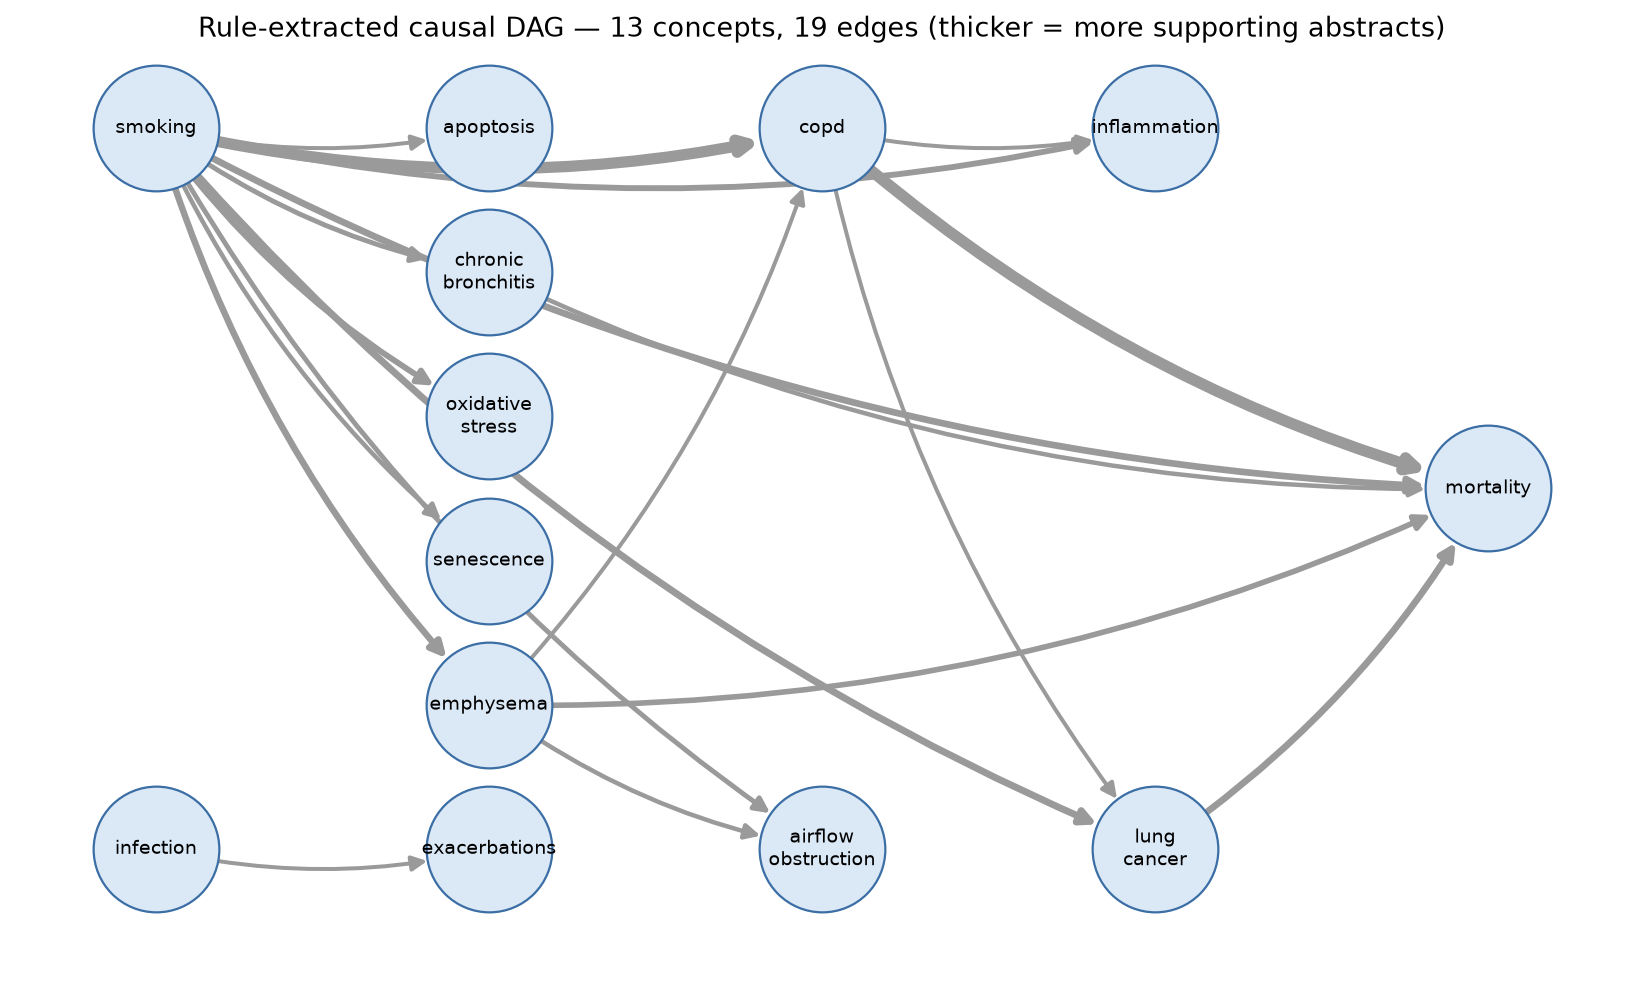
\includegraphics[width=0.95\linewidth]{dag_rules.png}\\[0.2em]
{\small (a) Rules: 13 concepts, 19 edges.}\\[1.2em]
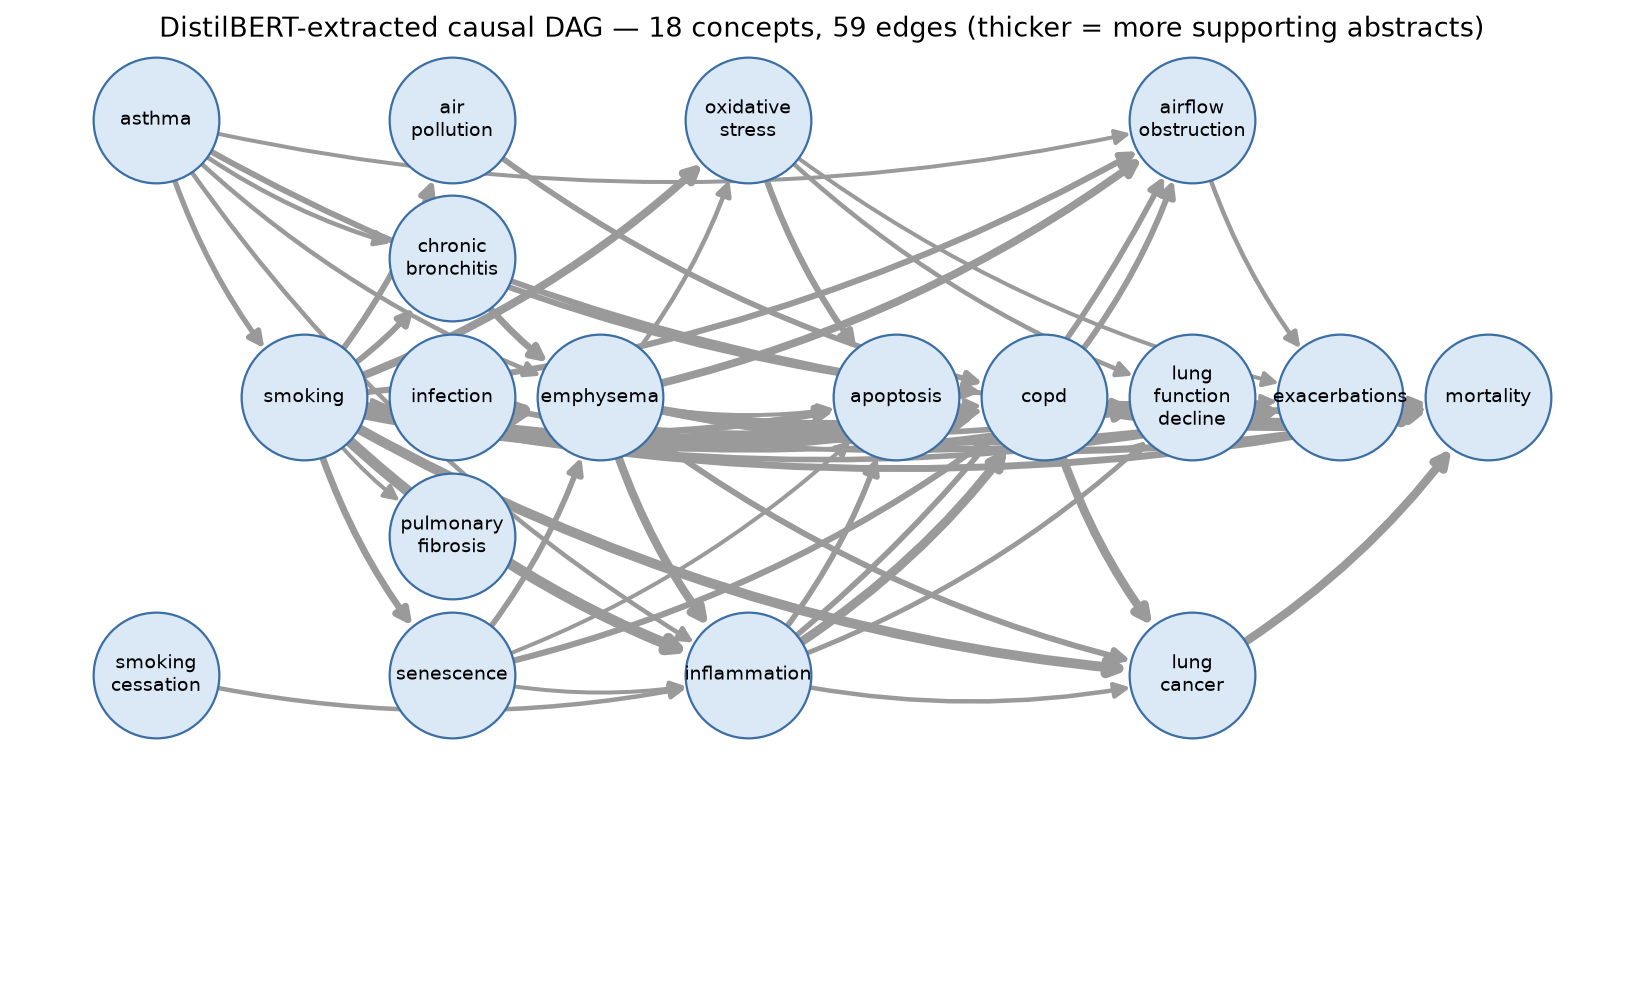
\includegraphics[width=0.95\linewidth]{dag_distilbert.png}\\[0.2em]
{\small (b) DistilBERT: 18 concepts, 59 edges.}
\caption{Final DAGs extracted from the same 500 PubMed abstracts. Columns follow the causal order; thicker arrows have more
supporting abstracts.}
\label{fig:dags}
\end{figure}

\begin{table}[H]
\centering\small
\begin{tabular}{@{}lcccccc@{}}
\toprule
DAG & Edges & Established & Unverified & Contradicts & Edge precision & Facts recovered \\
\midrule
Rules & 19 & 11 & 8 & \textbf{0} & \textbf{0.58} & 11 / 14 \\
DistilBERT & 59 & 13 & 44 & 2 & 0.22 & \textbf{13 / 14} \\
\bottomrule
\end{tabular}
\caption{Graph evaluation against 14 Surgeon General conclusions. DistilBERT's contradicting edges are smoking $\rightarrow$ air
pollution and asthma $\rightarrow$ smoking.}
\label{tab:graphs}
\end{table}

\subsection{Testing the structure on NHANES}

\begin{table}[H]
\centering\small
\begin{tabular}{@{}lc@{}}
\toprule
Candidate structure & BIC (higher is better) \\
\midrule
No arrows & $-46{,}728$ \\
Text arrows only & $-45{,}740$ \\
Age arrows only & $-45{,}276$ \\
Text + age (rules DAG) & $-45{,}058$ \\
Text + age (DistilBERT DAG) & $\mathbf{-45{,}045}$ \\
\bottomrule
\end{tabular}
\caption{Fit of alternative structures to the NHANES data.}
\label{tab:bic}
\end{table}

The extracted arrows add information beyond age (Table~\ref{tab:bic}). Of the four conditional independences implied by the rules
graph, two are rejected ($p < 10^{-90}$): chronic bronchitis is strongly associated with COPD and with emphysema even within the same
age and smoking group. Clinically, chronic bronchitis and emphysema are the two main forms of COPD. Papers express this with
\textit{includes} rather than causal wording, so neither extractor captured it as a cause--effect pair. The DistilBERT graph fits
slightly better because it contains chronic bronchitis $\rightarrow$ emphysema. We reported these rejections and did not add the edges by hand.

\subsection{Seeing versus doing}

\begin{table}[H]
\centering\small
\begin{tabular}{@{}lccccccc@{}}
\toprule
 & \multicolumn{2}{c}{Never} & \multicolumn{2}{c}{Former} & \multicolumn{2}{c}{Current} & Causal RR \\
\cmidrule(lr){2-3}\cmidrule(lr){4-5}\cmidrule(lr){6-7}
Outcome (\%) & see & do & see & do & see & do & current / never \\
\midrule
COPD & 1.02 & 1.12 & 7.16 & 5.24 & 8.86 & 10.42 & 9.3 \\
Emphysema & 0.35 & 0.37 & 3.89 & 2.82 & 4.36 & 5.35 & 14.3 \\
Chronic bronchitis & 3.57 & 3.73 & 8.02 & 7.25 & 10.61 & 10.87 & 2.9 \\
Lung cancer & 0.08 & 0.09 & 0.93 & 0.62 & 0.45 & 0.57 & 6.6 \\
Mortality & 3.48 & 3.85 & \textbf{9.33} & \textbf{6.40} & \textbf{5.54} & \textbf{6.93} & 1.8 \\
\bottomrule
\end{tabular}
\caption{Observational $P(Y \mid \text{smoking})$ (``see'') versus interventional $P(Y \mid \doop(\text{smoking}))$ (``do''), with RR the
causal risk ratio. The network's ``see'' values match the raw survey rates to within 0.2 percentage points.}
\label{tab:seedo}
\end{table}

Observationally, former smokers die more often than current smokers (9.3\% vs.\ 5.5\%), which would suggest that quitting is harmful.
Former smokers are much older on average. Under $\doop(\cdot)$, every group has the population's age distribution, and the order
reverses (6.4\% vs.\ 6.9\%). The same adjustment lowers the apparent COPD risk of former smokers and raises that of current smokers.

\subsection{Documented causal queries}

\begin{table}[H]
\centering\small
\begin{tabularx}{\linewidth}{@{}lYYl@{}}
\toprule
 & Question & Formal query & Answer \\
\midrule
Q1 & How much more COPD if everyone smoked vs.\ nobody? & $\frac{P(\text{copd}\mid\doop(\text{current}))}{P(\text{copd}\mid\doop(\text{never}))}$ & 9.3$\times$ \\
Q2 & Share of COPD that would not exist if nobody had smoked & $\frac{P(\text{copd})-P(\text{copd}\mid\doop(\text{never}))}{P(\text{copd})}$ & 72\% \\
Q3 & COPD risk, former vs.\ current smokers (same age mix) & $P(\text{copd}\mid\doop(\cdot))$ & 5.2\% vs.\ 10.4\% \\
Q4 & Effect of smoking on lung cancer & risk ratio under $\doop$ & 6.6$\times$ \\
Q5 & Effect of smoking on death during follow-up & risk ratio under $\doop$ & 1.8$\times$ \\
Q6 & Effect of COPD on death during follow-up & $P(\text{death}\mid\doop(\text{copd}{=}\text{yes}))$ vs.\ $\doop(\text{no})$ & 8.2\% vs.\ 4.8\% \\
\bottomrule
\end{tabularx}
\caption{Interventional queries answered by the fitted network. The directions of Q1, Q4, Q5 and Q6 agree with Surgeon General
conclusions~\citep{sgr2014}; the sources state that these effects exist, not their exact size.}
\label{tab:queries}
\end{table}

\subsection{How much does the extracted structure matter?}

Fitting the network on the DistilBERT DAG instead of the rules DAG leaves the smoking queries essentially unchanged (Q1 9.32 vs.\ 9.32;
Q5 1.80 vs.\ 1.78). In both graphs, age is smoking's only parent, so the adjustment set is the same. Errors \emph{below} a cause do not
change its total effect. Errors \emph{into} a cause do: in a network over age, smoking and COPD, reversing the single arrow to COPD
$\rightarrow$ smoking turns the causal risk ratio of smoking on COPD from \textbf{9.3} into \textbf{1.0}. Under that graph,
intervening on smoking cannot affect something that precedes it. The two structures are Markov equivalent and fit the data equally well,
so the data cannot choose between them. DistilBERT supported the reversed arrow in 33 abstracts, and cycle breaking rejected it only because the correct
direction had more support (104 abstracts).

\subsection{Fixing domain shift with labelled PubMed pairs}

The diagnostics above suggest one remedy for both failure modes: train on scientific text, and show the model sentences in which one
pair is causal and another is not. We therefore labelled a second PubMed sample for \emph{training}.

\textbf{Sample.} All 192 abstracts that contribute to the 300 evaluation pairs were excluded. From the remaining 304 abstracts, whole
abstracts were drawn at random (seed 42) until about 1{,}000 pairs were reached, and \emph{every} candidate pair of every sentence was
kept: 1{,}001 pairs from 397 sentences of 105 abstracts. The split is by abstract: 89 abstracts (780 pairs) for training and 16
(221 pairs) for validation. They were labelled with the same guideline and labeller as the 300 evaluation pairs, blind to all predictions;
152 pairs (15\%) are causal, and 43 sentences contain both a causal and a non-causal pair.

\textbf{Training.} A fresh DistilBERT was fine-tuned with the recipe of Section~\ref{sec:dl} on SemEval train plus the 780 PubMed pairs, and the
epoch was chosen by F1 on the 221 PubMed validation pairs (epoch 3, F1 0.69; the original model scores 0.49 on the same pairs). Long
PubMed sentences exhausted the memory of an 8\,GB laptop at batch size 32, so gradients were accumulated over four mini-batches of
eight. This keeps 32 sentences per update and reduces peak memory to about a quarter.

\begin{table}[H]
\centering\small
\begin{tabular}{@{}lcc@{}}
\toprule
 & Original DistilBERT & + 780 PubMed pairs \\
\midrule
SemEval test F1 [95\% CI] & 0.91 [0.88, 0.93] & \textbf{0.92} [0.89, 0.94] \\
PubMed precision / recall & 0.45 / 0.42 & \textbf{0.66} / \textbf{0.46} \\
PubMed F1 [95\% CI] & 0.43 [0.36, 0.52] & \textbf{0.54} [0.44, 0.65] \\
False alarms (est., of 6{,}051) & 744 & \textbf{357} \\
Wrong direction (est., of 6{,}051) & 23 & \textbf{10} \\
Pairs called causal, sentences with 7+ concepts & 24\% & \textbf{19\%} \\
Edges removed to break cycles & 59 & \textbf{37} \\
Graph edge precision & 0.22 & \textbf{0.29} \\
Edges contradicting the sources & \textbf{2} & 4 \\
\bottomrule
\end{tabular}
\caption{The DL model before and after adding labelled PubMed pairs. PubMed scores use the same 300 evaluation pairs and weights as
Table~\ref{tab:pubmed}.}
\label{tab:fix}
\end{table}

Precision on PubMed rises by 0.21 and the estimated false alarms halve, without any loss on SemEval (Table~\ref{tab:fix}). Pair
confusion is reduced but not solved: the share of pairs called causal now falls as sentences get more crowded, but stays well above the
rules. The graph needs fewer edges removed, and its edge precision rises, but two new edges contradict the sources (\textit{mortality
$\rightarrow$ chronic bronchitis} and \textit{COPD $\rightarrow$ oxidative stress}). Support for the reversed arrow \textit{COPD
$\rightarrow$ smoking} drops from 33 to 17 abstracts, against 149 for the correct direction. The causal answers are unchanged (Q1 9.32,
Q4 6.57, Q5 1.77). Two caveats apply: the bootstrap intervals still overlap, and the same labeller produced both the training and the
evaluation labels, so part of the gain may reflect learning the labeller's conventions.

\section{Discussion}

\textbf{The extractors trade precision for recall, and neither is enough alone.} On in-domain text the fine-tuned model is clearly
better. On scientific text, it recovers about three times as many causal pairs as the rules but adds more false alarms than correct
calls. The rules are precise but blind to most phrasings. For a graph that feeds causal reasoning, precision matters more than recall:
an unverified extra edge is a nuisance, while a reversed edge into a cause invalidates the answer.

\textbf{The symbolic stage provides what extraction cannot.} Exactly as the project brief anticipated, the extracted relations alone
were inconsistent: both directions for the same pair, edges contradicting established facts, and confidence scores that did not reflect
correctness. Acyclicity enforcement, evidence tracking, support thresholds and tests against data turned them into a usable structure.
Interventional queries answered on that structure separate the effect of smoking from that of age, which observational percentages,
and text that reports them, conflate.

\section{Limitations}

\begin{itemize}
  \item PubMed labels are \emph{silver} labels from an instruction model. It was evaluated against human labels on SemEval
        ($\kappa = 0.93$), but no human checked the PubMed sample, and the edge review files were not completed by a human reviewer.
  \item The reference list holds 14 conclusions, so ``unverified'' edges (e.g.\ mechanistic links such as apoptosis) may still be true.
  \item NHANES diagnoses are self-reported, mortality follow-up is short (about 1--7 years), and lung cancer is rare (54 cases), so Q4 is
        uncertain. Age is the only confounder modelled; income, occupational exposure and pollution are not.
  \item In the domain-shift fix, the same labeller produced the PubMed training and evaluation labels, which may flatter the
        retrained model; 300 evaluation pairs also leave the F1 intervals overlapping.
  \item Cycle breaking keeps the better-supported direction, which can fail when the wrong direction is stated more often.
\end{itemize}

\section{Conclusion and future work}

Fine-tuned transformers read causal language well, but on their own they do not produce a causal model that can be trusted. Combining
them with a symbolic stage that enforces structure, keeps evidence, tests against data and answers $\doop$-queries yields answers that
agree with the published evidence and avoid the confounding that misleads raw observation. Retraining with labelled PubMed pairs, several per sentence and split
by abstract, narrowed the domain gap (PubMed F1 0.43 to 0.54). Future work: (1) human labels for the PubMed training and evaluation pairs;
(2) a biomedical starting model such as PubMedBERT; (3) complete human review of the extracted edges and of a sample of the silver labels; and (4) add confounders
and spirometry-based airflow obstruction (NHANES 2007--2012) to the network.

\paragraph{Reproducibility.} All code is in one notebook (\texttt{causal\_nlp.ipynb}) with a fixed seed. Every download is cached, and package
versions are pinned in a full lock file. Steps 1--6 were re-run from scratch in a freshly built environment and reproduced every reported number; the domain-shift fix
(Step 7) was re-run end to end from the cached model.

\begin{thebibliography}{99}
\setlength{\itemsep}{2pt}
\small

\bibitem[Ankan and Panda(2015)]{ankan2015}
A.~Ankan and A.~Panda.
\newblock pgmpy: Probabilistic graphical models using Python.
\newblock In \emph{Proceedings of the 14th Python in Science Conference (SciPy)}, 2015.

\bibitem[Baldini~Soares et~al.(2019)]{baldinisoares2019}
L.~Baldini~Soares, N.~FitzGerald, J.~Ling, and T.~Kwiatkowski.
\newblock Matching the blanks: Distributional similarity for relation learning.
\newblock In \emph{Proceedings of ACL}, 2019.

\bibitem[Cohen(1960)]{cohen1960}
J.~Cohen.
\newblock A coefficient of agreement for nominal scales.
\newblock \emph{Educational and Psychological Measurement}, 20(1):37--46, 1960.

\bibitem[Devlin et~al.(2019)]{devlin2019}
J.~Devlin, M.-W. Chang, K.~Lee, and K.~Toutanova.
\newblock {BERT}: Pre-training of deep bidirectional transformers for language understanding.
\newblock In \emph{Proceedings of NAACL-HLT}, pages 4171--4186, 2019.

\bibitem[Efron(1979)]{efron1979}
B.~Efron.
\newblock Bootstrap methods: Another look at the jackknife.
\newblock \emph{The Annals of Statistics}, 7(1):1--26, 1979.

\bibitem[Heckerman et~al.(1995)]{heckerman1995}
D.~Heckerman, D.~Geiger, and D.~M. Chickering.
\newblock Learning {B}ayesian networks: The combination of knowledge and statistical data.
\newblock \emph{Machine Learning}, 20:197--243, 1995.

\bibitem[Hendrickx et~al.(2010)]{hendrickx2010}
I.~Hendrickx, S.~N. Kim, Z.~Kozareva, P.~Nakov, D.~{\'O}~S{\'e}aghdha, S.~Pad{\'o}, M.~Pennacchiotti, L.~Romano, and S.~Szpakowicz.
\newblock {SemEval}-2010 task 8: Multi-way classification of semantic relations between pairs of nominals.
\newblock In \emph{Proceedings of the 5th International Workshop on Semantic Evaluation}, pages 33--38, 2010.

\bibitem[Jin et~al.(2024)]{jin2024corr2cause}
Z.~Jin, J.~Liu, Z.~Lyu, S.~Poff, M.~Sachan, R.~Mihalcea, M.~Diab, and B.~Sch{\"o}lkopf.
\newblock Can large language models infer causation from correlation?
\newblock In \emph{International Conference on Learning Representations (ICLR)}, 2024.

\bibitem[Loshchilov and Hutter(2019)]{loshchilov2019}
I.~Loshchilov and F.~Hutter.
\newblock Decoupled weight decay regularization.
\newblock In \emph{International Conference on Learning Representations (ICLR)}, 2019.

\bibitem[NCHS(2022)]{nchsmort}
National Center for Health Statistics.
\newblock Public-use linked mortality files (NHANES, mortality follow-up through 2019).
\newblock \url{https://ftp.cdc.gov/pub/Health_Statistics/NCHS/datalinkage/linked_mortality/}.

\bibitem[CDC/NCHS(2013--2018)]{nhanes}
Centers for Disease Control and Prevention, National Center for Health Statistics.
\newblock National Health and Nutrition Examination Survey data, cycles 2013--2014, 2015--2016, 2017--2018.
\newblock \url{https://wwwn.cdc.gov/nchs/nhanes/}.

\bibitem[Pearl(1988)]{pearl1988}
J.~Pearl.
\newblock \emph{Probabilistic Reasoning in Intelligent Systems: Networks of Plausible Inference}.
\newblock Morgan Kaufmann, 1988.

\bibitem[Pearl(2009)]{pearl2009}
J.~Pearl.
\newblock \emph{Causality: Models, Reasoning, and Inference}.
\newblock Cambridge University Press, 2nd edition, 2009.

\bibitem[Sanh et~al.(2019)]{sanh2019}
V.~Sanh, L.~Debut, J.~Chaumond, and T.~Wolf.
\newblock {DistilBERT}, a distilled version of {BERT}: Smaller, faster, cheaper and lighter.
\newblock \emph{arXiv preprint arXiv:1910.01108}, 2019.

\bibitem[Schwarz(1978)]{schwarz1978}
G.~Schwarz.
\newblock Estimating the dimension of a model.
\newblock \emph{The Annals of Statistics}, 6(2):461--464, 1978.

\bibitem[USDHHS(2010)]{sgr2010}
U.S. Department of Health and Human Services.
\newblock \emph{How Tobacco Smoke Causes Disease: The Biology and Behavioral Basis for Smoking-Attributable Disease. A Report of the
Surgeon General}.
\newblock Atlanta, GA, 2010. \url{https://www.ncbi.nlm.nih.gov/books/NBK53021/}.

\bibitem[USDHHS(2014)]{sgr2014}
U.S. Department of Health and Human Services.
\newblock \emph{The Health Consequences of Smoking---50 Years of Progress. A Report of the Surgeon General}.
\newblock Atlanta, GA, 2014. \url{https://www.ncbi.nlm.nih.gov/books/NBK294322/}.

\bibitem[Wolf et~al.(2020)]{wolf2020}
T.~Wolf, L.~Debut, V.~Sanh, J.~Chaumond, C.~Delangue, A.~Moi, P.~Cistac, T.~Rault, R.~Louf, M.~Funtowicz, et~al.
\newblock Transformers: State-of-the-art natural language processing.
\newblock In \emph{Proceedings of EMNLP: System Demonstrations}, pages 38--45, 2020.

\end{thebibliography}

\end{document}
